\documentclass[aspectratio=169,11pt]{beamer}
\usepackage[T1]{fontenc}
\usepackage{lmodern,amsmath,amssymb,mathtools,bm,booktabs,array,graphicx,tikz}
\usetikzlibrary{arrows.meta,positioning,calc,decorations.pathreplacing,patterns}
\definecolor{ink}{HTML}{17344D}\definecolor{accent}{HTML}{087E8B}\definecolor{pale}{HTML}{EDF5F5}\definecolor{gold}{HTML}{AD6B19}
\providecommand{\dd}{\,\mathrm{d}}\providecommand{\R}{\mathbb{R}}
\providecommand{\E}{\mathbb{E}}\providecommand{\Var}{\operatorname{Var}}
\providecommand{\Cov}{\operatorname{Cov}}\providecommand{\diag}{\operatorname{diag}}
\providecommand{\norm}[1]{\left\lVert#1\right\rVert}
\providecommand{\abs}[1]{\left|#1\right|}
\usefonttheme{professionalfonts}
\setbeamercolor{normal text}{fg=black,bg=white}
\setbeamercolor{frametitle}{fg=ink,bg=white}
\setbeamercolor{title}{fg=ink}\setbeamercolor{structure}{fg=accent}
\setbeamercolor{block title}{fg=ink,bg=pale}\setbeamercolor{block body}{fg=black,bg=pale!40}
\setbeamercolor{alerted text}{fg=accent}
\setbeamerfont{frametitle}{size=\Large,series=\bfseries}
\setbeamerfont{title}{size=\LARGE,series=\bfseries}
\setbeamertemplate{navigation symbols}{}
\setbeamersize{text margin left=.7cm,text margin right=.7cm}
\setbeamertemplate{frametitle}{\vspace{.18cm}\insertframetitle\par\vspace{.1cm}{\color{accent}\hrule height .6pt}\vspace{.12cm}}
\newcommand{\notestarget}{notes.pdf}\newcommand{\noteslabel}{Notes}
\setbeamertemplate{footline}{\hspace{.7cm}\color{ink}\scriptsize Mathematical Cardiology\quad\href{\notestarget}{\noteslabel}\hfill\insertframenumber\,/\,\inserttotalframenumber\hspace{.7cm}\vspace{.18cm}}
\setbeamercovered{invisible}
\hypersetup{pdfauthor={Zan Ahmad},pdftitle={Fetal pathways and signed junction balances},pdfpagemode=UseNone}
\begin{document}
\begin{frame}[plain]\vfill
{\small\color{accent} Mathematical Cardiology \quad Lecture 7}\par\medskip
{\raggedright\hyphenpenalty=10000\exhyphenpenalty=10000\LARGE\bfseries\color{ink} Fetal pathways and signed junction balances}\par\bigskip
Zan Ahmad\par\smallskip
{\small Fall 2023}\par\vfill\end{frame}
\renewcommand{\notestarget}{notes.pdf\#note-interpretation-of-the-grouped-network}
\begin{frame}[label=slide-two-shunts-change-the-routes-figure]{Two shunts change the routes}
\centering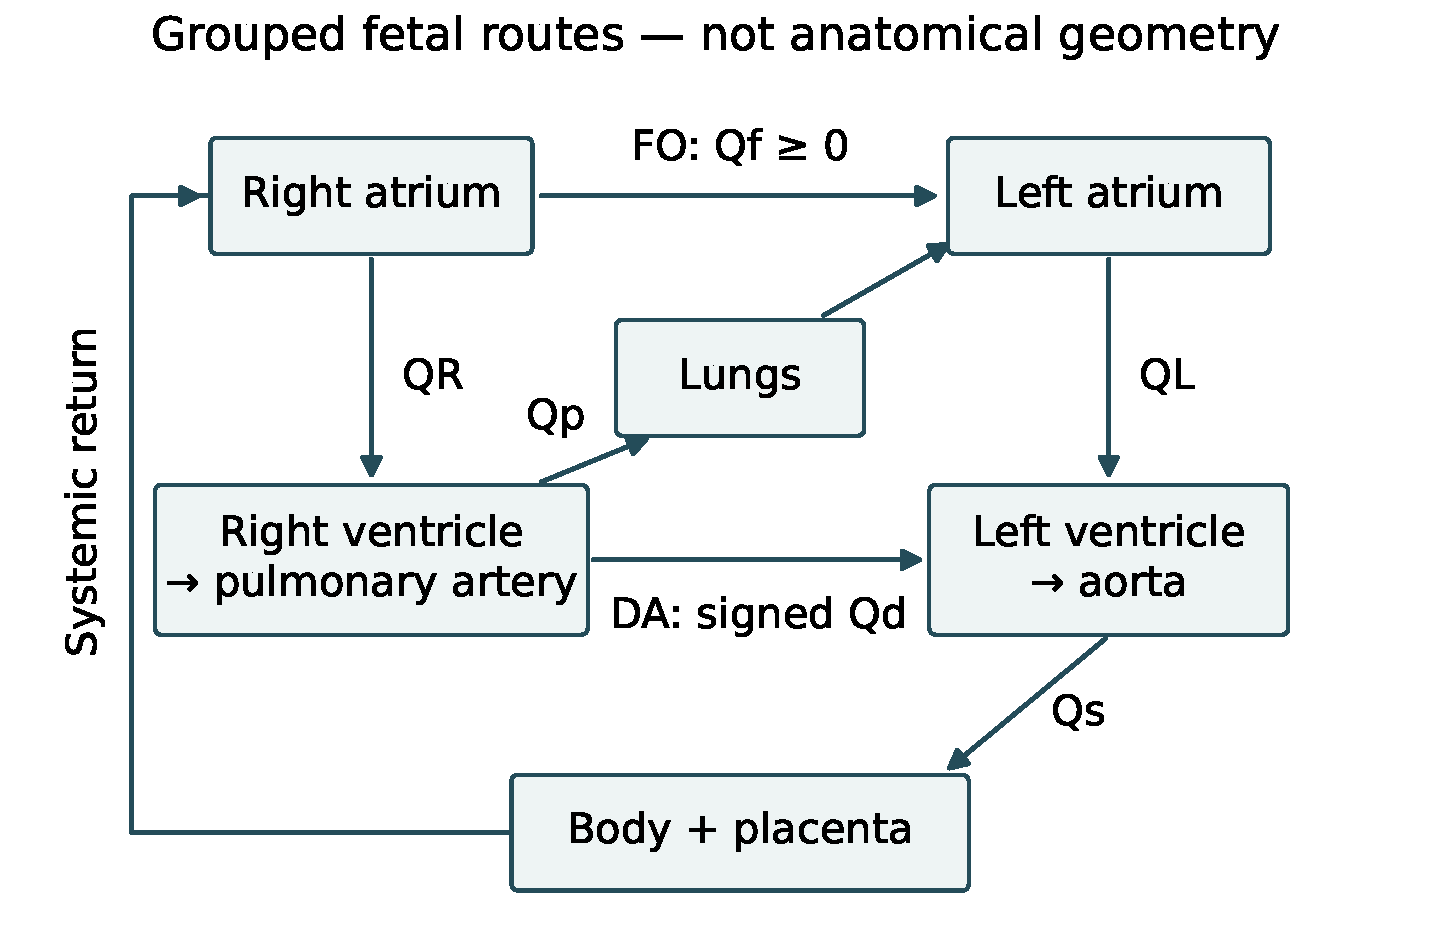
\includegraphics[width=.98\linewidth,height=.69\textheight,keepaspectratio]{fetal-routes.pdf}\end{frame}
\renewcommand{\notestarget}{notes.pdf\#note-interpretation-of-the-grouped-network}
\begin{frame}[t,fragile,label=slide-two-shunts-change-the-routes]{Two shunts change the routes}
Retain pulmonary flow $Q_p$ and grouped systemic flow $Q_s$.
\pause{}
The foramen ovale joins the atria; the ductus arteriosus joins pulmonary artery and aorta.

The placenta is an exchange interface, not free mixing of maternal and fetal blood.
\end{frame}
\renewcommand{\notestarget}{notes.pdf\#note-interpretation-of-the-grouped-network}
\begin{frame}[t,fragile,label=slide-declare-the-positive-directions]{Declare the positive directions}
\[Q_d>0:\quad\text{pulmonary artery}\longrightarrow\text{aorta}.\]
\[Q_f>0:\quad\text{right atrium}\longrightarrow\text{left atrium}.\]
\pause{}
A sign convention is not yet a one-way flow law.
\end{frame}
\renewcommand{\notestarget}{notes.pdf\#note-four-junctions-three-independent-equations}
\begin{frame}[t,fragile,label=slide-at-the-pulmonary-artery]{At the pulmonary artery}
Right-pump flow separates into two routes:
\[\boxed{Q_R=Q_p+Q_d}.\]
\pause{}
If $Q_p=100$ and $Q_d=50$, then $Q_R=150\,\mathrm{mL/min}$.
\end{frame}
\renewcommand{\notestarget}{notes.pdf\#note-four-junctions-three-independent-equations}
\begin{frame}[t,fragile,label=slide-at-the-left-atrium-and-aorta]{At the left atrium and aorta}
Pulmonary return and foramen flow enter the left side:
\[Q_L=Q_p+Q_f.\]
\pause{}
At the aortic junction,
\[Q_s=Q_L+Q_d.\]
\end{frame}
\renewcommand{\notestarget}{notes.pdf\#note-four-junctions-three-independent-equations}
\begin{frame}[t,fragile,label=slide-the-fourth-balance-is-not-independent]{The fourth balance is not independent}
\[Q_s=Q_L+Q_d=(Q_p+Q_f)+Q_d.\]
\pause{}
Rearrange the sum:
\[Q_s=(Q_p+Q_d)+Q_f=Q_R+Q_f.\]
The right-atrial balance follows from the other three.
\end{frame}
\renewcommand{\notestarget}{notes.pdf\#note-four-junctions-three-independent-equations}
\begin{frame}[t,fragile,label=slide-pump-output-need-not-equal-pulmonary-flow]{Pump output need not equal pulmonary flow}
For $(Q_p,Q_d,Q_f)=(100,50,40)$,
\[Q_R=150,\qquad Q_L=140,\qquad Q_s=190\,\mathrm{mL/min}.\]
\pause{}
Check both systemic balances:
\[140+50=190=150+40.\]
\end{frame}
\renewcommand{\notestarget}{notes.pdf\#note-a-reversible-ductus-and-a-one-way-foramen}
\begin{frame}[label=slide-an-open-ductus-can-reverse-figure]{An open ductus can reverse}
\centering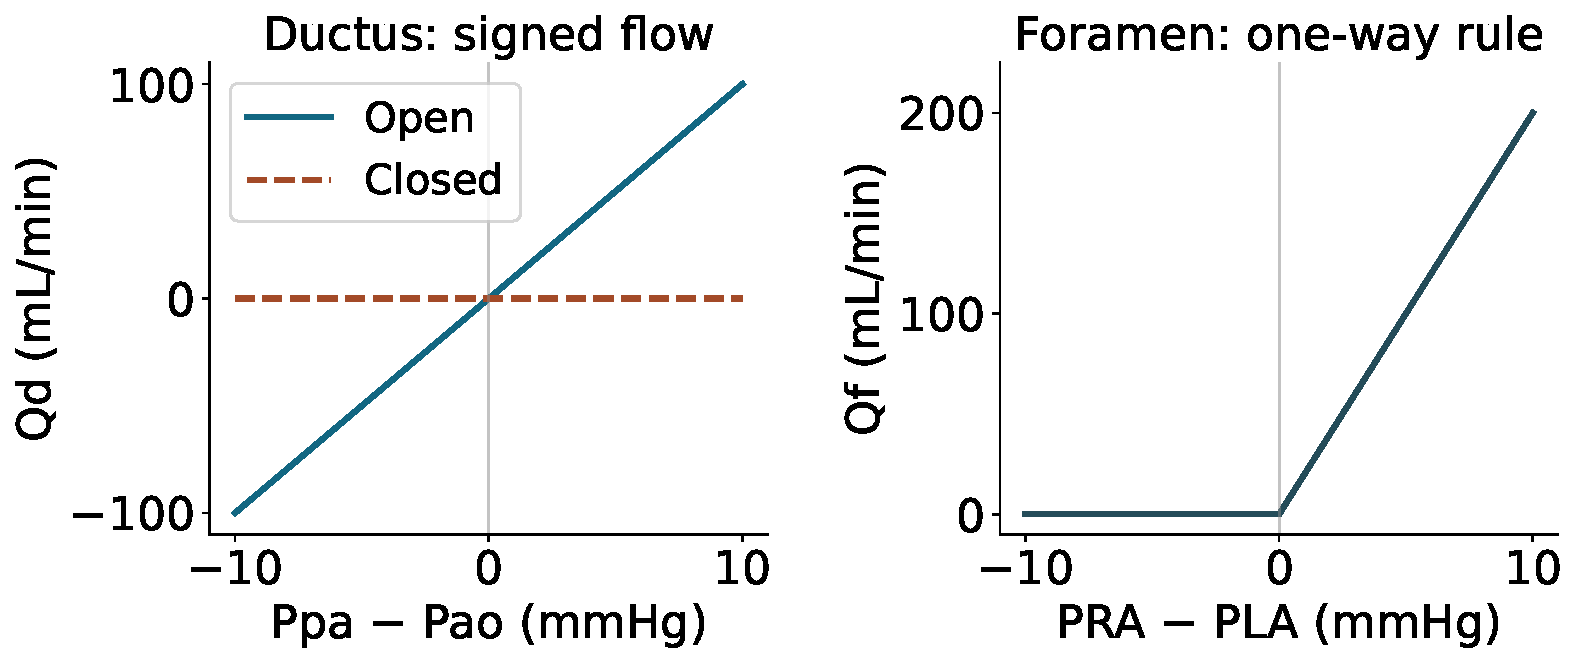
\includegraphics[width=.98\linewidth,height=.69\textheight,keepaspectratio]{shunt-rules.pdf}\end{frame}
\renewcommand{\notestarget}{notes.pdf\#note-a-reversible-ductus-and-a-one-way-foramen}
\begin{frame}[t,fragile,label=slide-an-open-ductus-can-reverse]{An open ductus can reverse}
\[Q_d=(P_{pa}-P_{ao})/R_d,\qquad R_d>0.\]
\pause{}
For $R_d=0.1$,
\[\frac{30-25}{0.1}=50,\qquad \frac{20-30}{0.1}=-100\,\mathrm{mL/min}.\]
The second case carries blood from aorta to pulmonary artery.
\end{frame}
\renewcommand{\notestarget}{notes.pdf\#note-a-reversible-ductus-and-a-one-way-foramen}
\begin{frame}[t,fragile,label=slide-a-one-way-rule-is-a-different-equation]{A one-way rule is a different equation}
\[Q_f=\frac{\max(P_{RA}-P_{LA},0)}{R_f}.\]
\pause{}
For $R_f=0.05$,
\[Q_f(6,4)=40,\qquad Q_f(4,7)=0\,\mathrm{mL/min}.\]
Forward resistance is finite in this surrogate.
\end{frame}
\renewcommand{\notestarget}{notes.pdf\#note-a-reversible-ductus-and-a-one-way-foramen}
\begin{frame}[t,fragile,label=slide-zero-flow-does-not-establish-closure]{Zero flow does not establish closure}
For a ductus,
\[Q_d=G_d(P_{pa}-P_{ao}).\]
\pause{}
$Q_d=0$ may mean $G_d=0$, or may mean equal boundary pressures.

Closure is zero conductance, not zero resistance.
\end{frame}
\renewcommand{\notestarget}{notes.pdf\#note-reversal-still-obeys-conservation}
\begin{frame}[t,fragile,label=slide-reversed-flow-enters-the-pulmonary-junction]{Reversed flow enters the pulmonary junction}
Take $Q_p=300$, $Q_d=-100$, $Q_f=0$.
\[Q_R=300-100=200.\]
\pause{}
The missing $100\,\mathrm{mL/min}$ arrives from the aorta through the ductus.
\end{frame}
\renewcommand{\notestarget}{notes.pdf\#note-reversal-still-obeys-conservation}
\begin{frame}[t,fragile,label=slide-the-aortic-balance-agrees]{The aortic balance agrees}
\[Q_L=300+0=300,\qquad Q_s=300-100=200.\]
\pause{}
Of the left-pump output, $100$ returns to the pulmonary route and $200$ enters the systemic route.

No blood is created by the negative sign.
\end{frame}
\renewcommand{\notestarget}{notes.pdf\#note-reversal-still-obeys-conservation}
\begin{frame}[t,fragile,label=slide-conservation-leaves-freedom]{Conservation leaves freedom}
Choose $Q_p$, $Q_d$, $Q_f$; then
\[\begin{pmatrix}Q_R\\Q_L\\Q_s\end{pmatrix}
=\begin{pmatrix}Q_p+Q_d\\Q_p+Q_f\\Q_p+Q_f+Q_d\end{pmatrix}.\]
\pause{}
Conservation determines the remaining flows, but does not choose the first three.
\end{frame}
\renewcommand{\notestarget}{notes.pdf\#note-reversal-still-obeys-conservation}
\begin{frame}[t,fragile,label=slide-pressure-rules-do-not-solve-the-whole-circulation]{Pressure rules do not solve the whole circulation}
The companion prescribes local pressures and illustrative pulmonary flows.
\pause{}
A full model must also determine those pressures from chambers, vascular properties, boundary conditions and blood volume.
\end{frame}
\renewcommand{\notestarget}{notes.pdf\#note-changing-the-network-at-birth}
\begin{frame}[t,fragile,label=slide-the-transition-changes-both-pressures-and-routes]{The transition changes both pressures and routes}
Pulmonary conditions change; the placental route is removed.
\pause{}
Ductus flow can reverse while conductance remains positive.
Foramen flow can stop under an unfavorable pressure difference.

Neither event alone specifies anatomical closure time.
\end{frame}
\renewcommand{\notestarget}{notes.pdf\#note-changing-the-network-at-birth}
\begin{frame}[t,fragile,label=slide-recover-the-series-circulation-as-a-limit]{Recover the series circulation as a limit}
If $Q_d=Q_f=0$,
\[Q_R=Q_p,\qquad Q_L=Q_p,\qquad Q_s=Q_L.\]
\pause{}
\[\boxed{Q_R=Q_p=Q_L=Q_s}.\]
Deleting a shunt requires rebalancing the flows.
\end{frame}
\end{document}
